\chapter{Conception}
\begin{onehalfspace}

\newpage

\section{Base de donnée}



Odoo, comme toute autre application, a besoin d'une base de donnée \emph{PostgreSQL} pour persister des informations. Malheureusement, la communauté de Docker n'est pas si satisfaite vis-à-vis l'idée de containériser les bases de données. Nous allons prouver à travers deux scénarios qu'il serait une imprudence de tourner les bases de données dans des conteneurs.

Le fait de la rapidité et la légèreté de Docker et des conteneurs en général a poussé CoreOS d'adopter une certaine philosophie à l'égard de la gestion et l'ordonnancement des conteneurs. En effet, lorsqu'un conteneur s'est arrêté pour une raison quelconque, il va être automatiquement écrasé et remplacé par un nouveau qui va tourner le même service. Une philosophie, certes, moins prudente et parait naïve, mais sa simplicité épargne beaucoup de problèmes à tout le monde.

Par conséquent, on ne peut en aucun cas mettre les données dans le système de fichiers d'un conteneur sous peine de les perdre. La figure \ref{fig:database1} montre qu'après avoir tuer un conteneur, ses données sont perdues.

\begin{figure}[H]
\centering
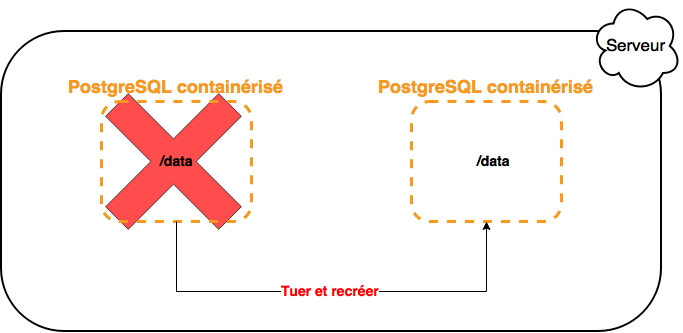
\includegraphics [scale=0.5]{chapitre4/assets/database1}
\caption{Données perdues - scénario 1}
\label{fig:database1}
\end{figure}

Pour y remédier, l'on peut penser à monter le volume des données dans le serveur hôte, ainsi les données sont plus ou moins persistantes. Outre le fait que les données seront certainement perdues quand le serveur tombe en panne, le conteneur n'aura plus accès aux données quand il sera réordonnancé. En effet, le caractère imprévisible de l'ordonnanceur \emph{Fleet} fait qu'il n'y a pas de garantie qu'un conteneur réside dans le même serveur. La figure \ref{fig:database2} montre ce scénario.

\begin{figure}[H]
\centering
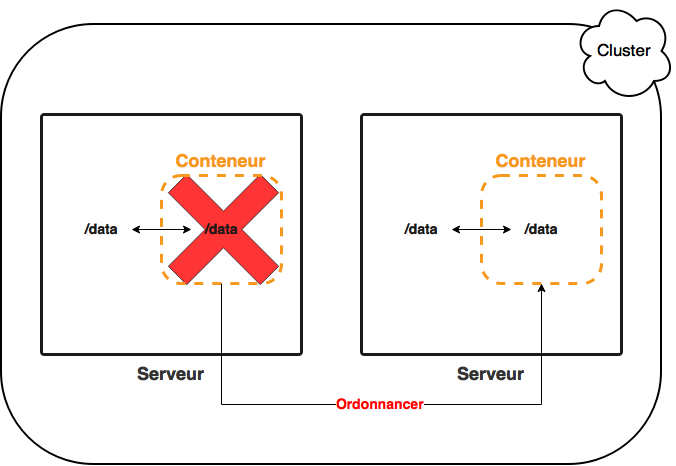
\includegraphics [scale=0.5]{chapitre4/assets/database2}
\caption{Données perdues - scénario 2}
\label{fig:database2}
\end{figure}


Dans un environnement de production, il est encore tôt pour mettre les bases de donnée et les applications à états (stateful) en général dans des conteneurs. De ce fait, il serait judicieux de les faire sortir de l'architecture à base de conteneurs. En effet, deux solutions se portent à nous, les bases de données vont être mis en place suivant l'informatique classique ou elles vont être consommées comme un service à partir d'une partie tierce cloud (Délégation de l'informatique). La dernière solution est coûteuse mais il est plus fiable.



\section{Scalabilité et disponibilité}


Parmi les contraintes qui ont poussé Sayoo à migrer vers le Cloud, c'est de garantir une haute disponibilité et une scalabilité infinie.

La haute disponibilité fait référence au fait qu'un service est en quelque sorte tolérant à une échec ou à une panne. Nous allons assurer cela en faisant la redondance des services dans différents serveurs du cluser.

La scalabilité ou l'évolutivité c'est la capacité d'une application à pouvoir exploiter des nouvelles ressources récemment déployées pour répondre à un pic de charge. En fait, la scalabilité n'est pas apporté par le Cloud, qui lui apporte l'élasticité, mais c'est l'application elle-même qui l'apporte. L'idée que toute application déployée dans un milieu élastique Cloud peut être évolutive est fausse.


Pour faire une bonne conception d'un \acrshort{saas} scalable, il faut distinguer d'abord deux types d'application:

\begin{itemize}
	\item Application \textbf{stateful} ou à états: C'est une application dont les processus ne stockent aucune donnée qui doit persister, même dans un temps aussi petit qu'il soit, dans son espace mémoire ou système de fichiers;
	\item Application \textbf{stateless} ou sans états: C'est une application qui stocke tous les données persistentes dans un service de support externe (Base de donnée, queue, mémoire cache, etc.).
\end{itemize}

Une application scalable doit être \textbf{stateless}, plus que cela, il doit respecter les douze-facteurs définies dans l'annexe \ref{annexe:12factors}. Une application scalable suppose qu'aucune donnée mise en cache (mémoire, disque) ne sera disponible dans une requête ultérieure. En effet, les chances sont élevées qu'une future requête sera servi par un processus différent du même service.


La figure \ref{fig:non-scalable} montre un service qui n'est évolutive contrairement au service présenté dans la figure \ref{fig:scalable}.


\begin{figure}[H]
\centering
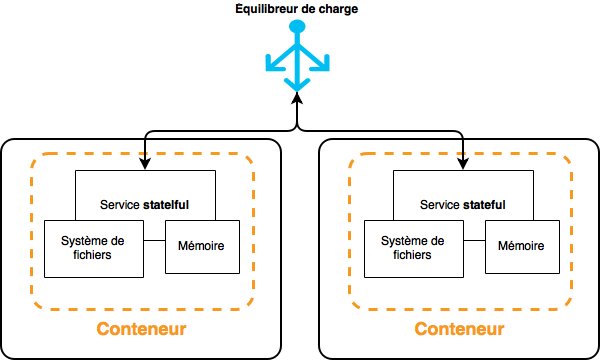
\includegraphics [scale=0.5]{chapitre4/assets/stateful}
\caption{Service non scalable}
\label{fig:non-scalable}
\end{figure}

\begin{figure}[H]
\centering
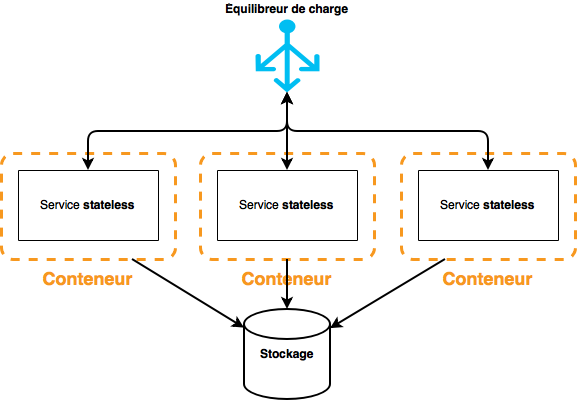
\includegraphics [scale=0.5]{chapitre4/assets/stateless}
\caption{Service scalable}
\label{fig:scalable}
\end{figure}


\section{Architecture}

\begin{figure}[H]
\centering
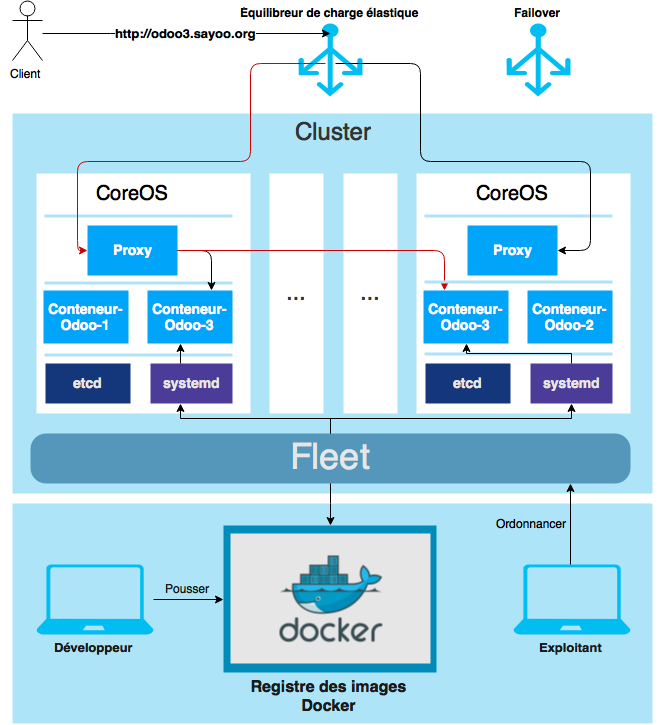
\includegraphics [scale=0.7]{chapitre4/assets/architecture}
\caption{Achitecture de la solution}
\label{fig:architecture}
\end{figure}

L'architecture est très simplifiée car on a fait abstraction du comportement internes des composants de CoreOS. Elle décrit trois processus et implique trois acteurs:


\begin{itemize}
 	\item Développeur: Il développe, personnalise et adapte l'image Odoo de base aux besoin du client. Une fois le développement est fait, le développeur pousse l'image Odoo vers le registre des images de Docker. Cette image est étiquetée par un nom, une version et un environnement (développement, test, production);
 	\item Exploitant: Il exploite l'ordonnanceur Fleet pour déployer l'application que le développeur vient de pousser dans le registre. L'exploitant va demander à l'ordonnanceur, par exemple, de lancer le service en mode haute disponibilité. L'ordonnanceur lance plusieurs instances du service dans des serveurs différents. L'exploitant, remarquant un pic de charge sur ce service, va demander de lancer une autre instance qui compense la surcharge;
 	\item Client: C'est l'utilisateur final de l'application. Il va saisir l'\acrshort{url} de son application. Son requête va être intercepté par l'équilibreur de charge qui va faire suivre la demande à un des serveurs du cluster. Quand la requête est arrivée, il tombe sur le proxy de ce serveur qui va faire suivre la requête à l'instance du service la moins chargée, quitte même à la faire suivre vers une instance dans un autre serveur.
 \end{itemize} 


L'idée c'est que une application doit être capable d'envoyer les réponses de façon consistante à partir de n'importe instance exécutant l'application.********


\end{onehalfspace}
